\section{Metodología de la Investigación}

Para el desarrollo del trabajo de grado, se propuso un modelo de prototipado iterativo compuesto de 5 fases (Ver fig. \ref{fig:met}), que permitió avanzar a medida que se fue completando la fase anterior y permitió el poder iterar sobre lo que se ha desarrollado anteriormente.

\begin{figure}[H]
    \centering
    \caption{\\Metodología de investigación}
    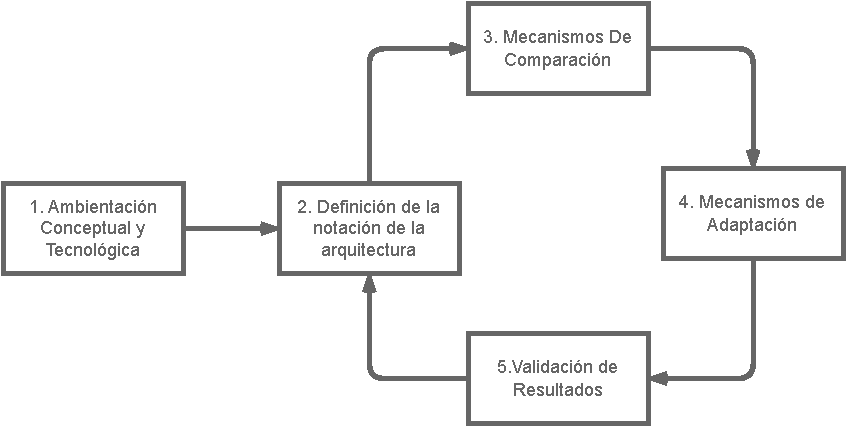
\includegraphics[width=0.7\linewidth]{images/Metodologia.pdf}
    \label{fig:met}
\end{figure}

\subsection{Ambientación Conceptual y Tecnológica}

La primera fase de la metodología se basó en la revisión de la literatura, al igual que de lo presente en la industria, lo anterior fué necesario para cubrir las bases tanto conceptuales como técnicas requeridas para el desarrollo del proyecto. 

\subsubsection*{Actividades}

\begin{enumerate}
    \itemsep-2mm
    \item Identificación de las características principales de un sistema auto-adaptable.
    \item Análisis de los mecanismos de adaptación de la arquitectura.
    \item Análisis los algoritmos empleados para la comparación de las arquitecturas.
    \item Determinación de los criterios de selección para el lenguaje de notación.
    \item Evaluación de los posibles lenguajes de programación para la implementación a realizar.
\end{enumerate} 

\subsubsection*{Productos}

\begin{enumerate}
    \itemsep-2mm
    \item Lista de criterios de selección para el lenguaje de notación.
    \item Evaluación de los posibles lenguajes de programación para la implementación.
\end{enumerate}

\subsection{Definición de la notación de la arquitectura}

La segunda fase consistió en la definición del cómo se realiza la declaración de la arquitectura. Partiendo de los criterios de selección establecidos en la fase 1, se determinó un lenguaje de notación el cual permitió definir la arquitectura objetivo a alcanzar, al igual que la gramática correspondiente para poder realizar dicha declaración. 

\subsubsection*{Actividades}

\begin{enumerate}
    \itemsep-2mm
    \item Selección del lenguaje de marcado a usar a partir de los criterios establecidos.
    \item Definición de la gramática a usar para la definición de la arquitectura.
    \item Determinación de como se realizará la representación de los componentes y partes de la arquitectura.
    \item Implementación de una validador de la notación propuesta.
\end{enumerate}    

\subsubsection*{Productos}

\begin{enumerate}
    \itemsep-2mm
    \item Notación a usar para la declaración de los requerimientos de las aplicaciones.
    \item Validador de los archivos de configuración de la notación definida
\end{enumerate}

\subsection{Mecanismos De Comparación}

Durante la tercera fase del proyecto, se buscó determinar e implementar cómo se realiza la comparación entre el estado de la arquitectura obtenido durante la auto-descripción de la misma y el objetivo establecido. Así mismo, y con el fin de reportar a los administradores de los sistemas, también fue necesario definir los \textit{niveles} de similitud entre las 2 arquitecturas.

\subsubsection*{Actividades}

\begin{enumerate}
    \itemsep-2mm
    \item Selección del mecanismo de comparación a usar para evaluación de estado de la arquitectura.
    \item Implementación del mecanismo de comparación seleccionado.
    \item Determinación de los diferentes niveles de similitud entre arquitecturas.
\end{enumerate}    

\subsubsection*{Productos}

\begin{enumerate}
    \itemsep-2mm
    \item Implementación de un mecanismos que permita establecer el estado del sistema.
    \item Implementación de una comparación entre el estado de referencia y el estado actual.
\end{enumerate}

\subsection{Mecanismos De Adaptación}

La cuarta fase del proyecto fue orientada a la selección, al igual que la implementación en Smart Campus UIS, del conjunto de mecanismos de adaptación de la arquitectura. 

\subsubsection*{Actividades}

\begin{enumerate}
    \itemsep-2mm
    \item Definición el conjunto de mecanismos de adaptación.
    \item Implementación el conjunto de mecanismos de adaptación seleccionados.
\end{enumerate}  

\subsubsection*{Productos}

\begin{enumerate}
    \itemsep-2mm
    \item Implementación de un servicio encargado de la planeación para la ejecución de los mecanismos de adaptación definidos
    \item Implementación de un servicio encargado de la ejecución de las acciones planeadas.
\end{enumerate}

\subsection{Validación De Resultados}

La fase final del proyecto se centró principalmente en la realización de pruebas de los mecanismos implementados, los resultados obtenidos al igual que la documentación de todo lo que se desarrolló durante el proyecto.

\subsubsection*{Actividades}

\begin{enumerate}
    \itemsep-2mm
    \item Realización de las pruebas del funcionamiento de la implementación realizada con diversas arquitecturas objetivo.
    \item Recopilación la documentación generada durante el desarrollo de cada una de las fases del proyecto.
    \item Compilación de la documentación para generar el documento final.
    \item Correcciones y adiciones para la presentación final del proyecto de grado.
\end{enumerate}  

\subsubsection*{Productos}

\begin{enumerate}
    \itemsep-2mm
    \item Validación del funcionamiento de los mecanismos implementados.
    \item Código fuente de los diferentes servicios y librerías implementadas durante el transcurso del proyecto
    \item Documento final detallando el desarrollo del proyecto
    \item Presentación para la sustentación del proyecto
\end{enumerate}